\chapter{Introduction}\label{ch:introduction}
In most laboratories around the world, computers are in charge of controlling experiments. From complex systems such as particle accelerators to simpler UV-Vis spectrometers, there's always a computer that's responsible for asking the user for some input, performing a measurement, and displaying the results. Therefore, learning how to control devices with a computer is of the utmost importance for every experimentalist who wants to gain a deeper degree of freedom when planning measurements.

This book is task-oriented, meaning that it focuses on how things can be done and not so much on theory or on how programming works in general. This approach can lead to some generalizations that may not be correct in all scenarios. We ask your forgiveness in those cases and your cooperation: if you find anything that can be improved or corrected, please contact us\footnote{courses@pythonforthelab.com}.

Together with the book, there's a website\footnote{https://www.pythonforthelab.com} where you can find extra information, anecdotes, and examples that we couldn't fit here. Remember that the website and its forum are the proper places to communicate with fellow Python For The Lab readers. If you're stuck on any of the exercises or have questions that aren't answered in the book, don't hesitate to post in the forum. Continuous feedback is the best way to improve this book.

\section{What You're Going To Learn}\label{sec:what-are-you-going-to-learn}
\begin{center}
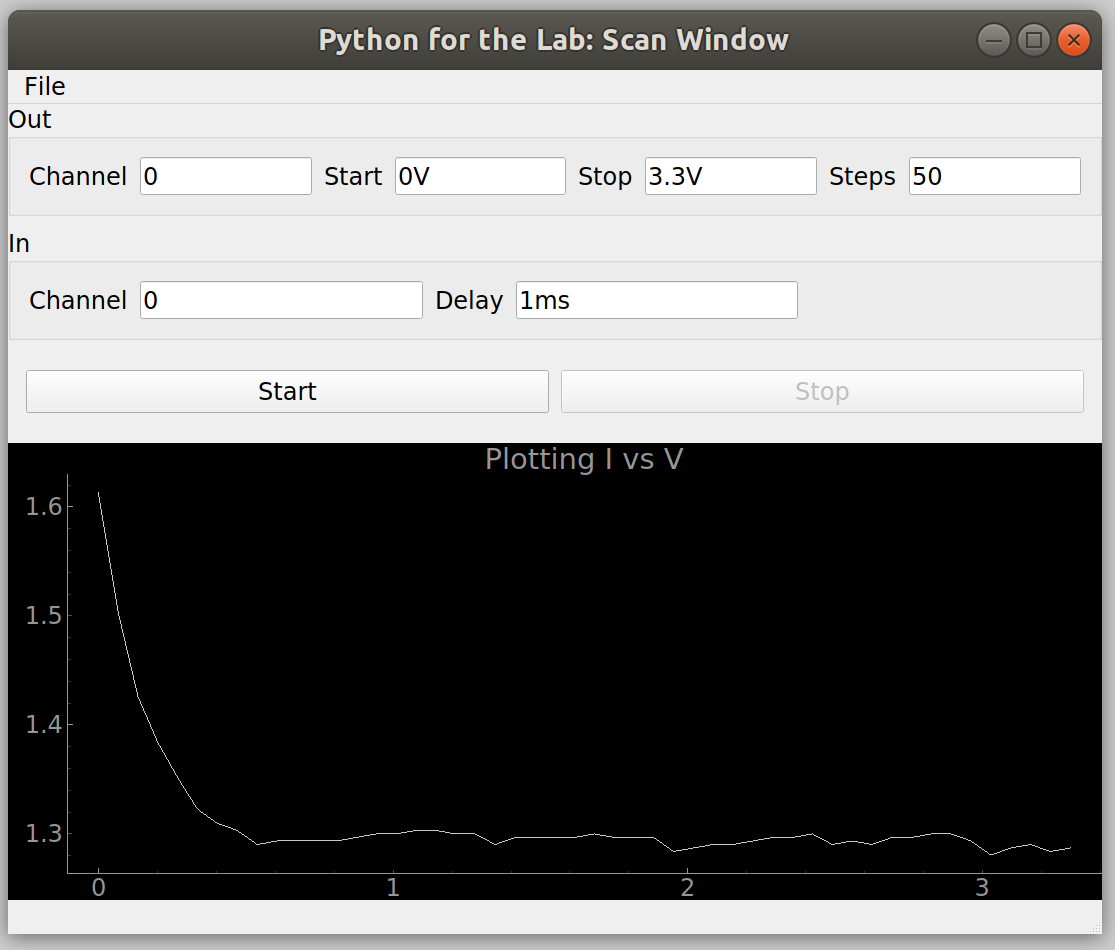
\includegraphics[width=.6\linewidth]{images/Chapter_01/screenshot.png}
\end{center}

This book is the result of many years of developing software for scientific applications and, more importantly, of several workshops organized in different universities and companies around Europe. In this time, we've gained experience developing new programs, and we've also collected invaluable feedback from students. With these two elements, we've designed the book to allow the reader to improve their Python proficiency while also showing a clear path to getting started with instrumentation software.

We crafted each chapter to introduce new Python topics alongside the specific tools needed to control a related experiment. For example, in Chapter~\ref{ch:first-driver} we develop a driver for a device and take a first dive into classes and objects. We introduce threads in Chapter~\ref{ch:run-experiment} when we discuss how to stop a running experiment. We also cover how to create user interfaces to accept user input and display data in real-time, such as in the image above. By following a task-oriented approach, students get the initial direction, tools, and vocabulary to ask for help if needed.

Regarding instrumentation itself, we've compiled what we believe are best practices that speed up the development of solutions and ensure a more prolonged survival of the programs. We discuss how to follow programming patterns that allow the exchange of solutions between people from the same lab or other parts of the world. This book is not a programmer's book, but a scientist's book written for another scientist. We try to use clear and concise language as much as possible, avoiding jargon where it's not necessary.

\section{Who This Book Is For}\label{sec:who-can-read-this-book}
We don't assume any proficiency in Python for readers looking to follow the book. We ask only that you have a grasp of \textit{if-statements}, \textit{for-loops}, \textit{while-loops}, and when to use them. You'll gain new knowledge when it's required through carefully planned examples and exercises. If you're already proficient in Python, we still believe there's value in the best practices we show, the structure of the code, and the way we decided to solve problems. There may be many paths, but the goal is the same: to extend the possibilities of an experiment by controlling it with custom software.

We believe that anybody working in a lab already has some knowledge of how to perform an experiment. The book proposes to measure the I-V curve of a diode. You don't need to understand the phenomenon; we use it as an example of an experiment in which one voltage is varied and another voltage is measured. This simple example is a building block of most experiments, like controlling temperatures, moving piezo-stages, or tuning a laser's frequency. By using an LED as the diode in the experiment, we can see the effect of applying a voltage.

\section{How to Obtain the PFTL DAQ Device}\label{sec:pftl-daq-device}
We've developed a device called the {PFTL DAQ} that works as a data acquisition board. The instructor provides these boards during the workshops, but if you acquired this book online and would like to buy one of these devices, please contact us\footnote{courses@pythonforthelab.com}. The devices are open source/open hardware and are based on the \textbf{Arduino DUE}. You can find the instructions for building one on our website. If you have access to any other acquisition card, you can adapt the course contents to your needs with a bit of tinkering.

Building software for the lab has a reality component that's not covered in any other books or tutorials. The fact that we are interacting with real-world devices, which can change an experiment's state, makes the development process much more compelling. The PFTL DAQ is a toy device so it's easy to replace, but it's also capable of performing quantitative measurements.

\subsection{What you'll need to build your acquisition device}
If you want to build the acquisition device, the main component you should source is an \textbf{Arduino DUE}. The official web store\footnote{https://www.arduino.cc} usually has them in stock. You can also check out other retailers such as eBay and AliExpress. If your budget allows for it, we strongly recommend getting an official board, since that's the best way to support the project.

In addition to the acquisition board, you'll also need a small protoboard, three jumper wires, one LED of any color you prefer, and a resistor of $100\,\Omega$ (although $220\,\Omega$ should also work fine). These components can easily be found in any electronics shop, both online or in store. If you work at a university or research institute, most labs will already have them in stock for you to borrow.

Once you have all the components, you can load the firmware onto the Arduino board. The code you'll need is freely available in our Github repository\footnote{https://github.com/PFTL/pythonforthelab}. If you encounter problems at any point, please don't hesitate to contact us. Our website has more information on how to get started with Arduino. We're also willing to answer your questions either via e-mail or on the forum.

\section{Why Build Your Own Software}\label{sec:why-building-your-software}
Computers and their software should be regarded as tools and not as obstacles in a researcher's daily tasks. However, when it comes to controlling a setup, many scientists prefer to be bound by the specifications of the software provided instead of pursuing innovative ideas. Once a researcher learns how to develop their own programs, these limitations fall and creativity can sprout. With automation, researchers can increase the throughput of the setup and reduce human error. Even experiments that were once impossible can become reachable by introducing smart feedback loops.

However, there's an added consideration to keep in mind while building software for research labs: reproducibility. It is a primary concern for modern scientists to be able to reproduce results and enable others to perform the same measurements. We believe that open-source software lowers the barrier to entry for newcomers and allows present and future colleagues to build on experience instead of reinventing the wheel. The practices we follow in the book are ideal for sharing entire programs or at least parts of them with the broad community.

\section{Why Use Python}\label{sec:why-python?}
Python has become ubiquitous in many research labs for several different reasons. First, Python is open source, and we firmly believe that the future of research lies in openness. Even for an industrial researcher, the results and the processes for generating data should be open to present and future colleagues. Python leverages the knowledge gathered in myriad areas to deliver a better product. Python can be found everywhere, from high-performance computing to machine learning, experiments, websites, and more.

Another factor to consider is that Python is free, so there's no overhead when it comes to implementing it. There's no limit to the number of machines on which you can install Python or the number of different simultaneous users you install it for. Moreover, there's a myriad of professionally-developed tools (such as NumPy, SciPy, and scikit-learn) that are also free for you to use. Anaconda, a popular data science platform, provides users with high-quality advice and troubleshooting, filling an often encountered gap in open-source software.

However, for experimentalists, there's a big downside when considering Python. Searching online for instructions on how to control an experiment yields few sources and even fewer if focusing on Python alone. Fortunately, this is changing thanks to an ever-growing number of people developing open-source code and writing handy documentation. Python can achieve all the same functionality of LabView. The only limitation is the existence of drivers for more sophisticated instruments. With a stronger community, companies will realize the value of providing those drivers for other programming environments.

But the choice of Python is not restricted to the lab. In many cases, Python is used for data analysis, and so it makes sense to bring its use to the source of the data, which is the experiment itself. Moreover, many more exciting things are possible with Python, like building websites, developing machine learning algorithms, and automatizing your daily tasks. Learning Python increases your odds of finding work both in and out of academia, and for both people who wish to continue working with experiments and those who want to focus on data analysis and beyond.

\section{How to Use the Onion Principle}\label{sec:onion-principle}
When we start developing software, it can be tough to think ahead. Most likely, we have a small problem that we want to solve as quickly as possible, and we just go for it. Later on, it may turn out that the "small problem" is something worth investigating a little deeper. Our software won't handle the new tasks, and we'll need to improve it. Having a proper set of rules in place will help us develop code that can adapt to our future needs while keeping us productive in the present. We like to call those rules the Onion Principle.

The rules we're talking about are not written in stone. You won't find them in any book (we haven't written them here, either). Instead, we're talking about a state of mind that empowers us to develop better, clearer, and more expandable code. Sitting down and reflecting is the best thing we can do, even moreso than sitting down and typing. When dealing with experiments, we have to ask ourselves may questions. What do we know? What do we need to prove how to do it? Only then can we sit down to write a program that responds to our needs.

If we build something that we cannot expand, then it will become useless very soon. When we don't know what may happen with our code, we should think ahead and structure it as an onion, in layers. This isn't something that occurs naturally, but we can develop our procedures to ensure that we're developing future-proof code. Once we get the hang of it, it will take much less time than being disorganized and not having the proper structure. We can avoid problems such as variables that aren't self-descriptive, lack of comments, and many more.

It's not all about being future-proof, though. When we start with a simple task, we want to solve it quickly. We don't want to spend hours developing useless lines of code just thinking \textit{what if}. This approach is known as \textit{premature optimization}. If we spend too much time trying to solve a problem that may appear, we might not see the issue that will arise. Therefore, it's better to fail quickly and improve than to fail later and run out of time.

However, having a strong foundation is always important. Taking shortcuts just because we don't want to create a separate file will give us more headaches, even in the short term. We should build code that is robust enough to support expansion later on. In the same way that we take several steps to perform an experiment, starting with the sample preparation, we should take steps when developing software, perhaps even starting with sample code.

In this book, we'll go from a one-off script that can get the job done in minutes to a fully-fledged user interface that will allow us to change the parameters of the experiment and visualize them in real-time.

\section{Where to Get the Code}\label{sec:where-to-get-the-code}
The code that you'll develop through the book is freely available on Github\footnote{https://github.com/PFTL/py4lab}. The code has been organized by chapters to make it more accessible while reading. There's also an extra folder with a version of the program that goes beyond what the book covers. For example, the code includes documentation and an installation script. In this way, readers can think of the possible directions to take for their software after they've finished with the book.

\sloppy If you have found any errors or would like to contact us, please send an e-mail to {aquiles@pythonforthelab.com}. We'll get back to you as soon as possible.

\section{How to Organize a Python for the Lab Workshop}\label{sec:organizing-a-python-for-the-lab-workshop}
Python for the Lab was born to bring unite researchers working in a lab with the Python programming language. With that goal in mind, we developed this book along with a workshop in which we can train scientists.

\sloppy If you would like to organize a Python for the Lab workshop at your institution, contact us by e-mail at {courses@pythonforthelab.com} to discuss the different options. You can also find more information about the courses on our website: {https://www.pythonforthelab.com}.
